\chapter{Approccio}
Recentemente sono stati sviluppati modelli linguistici pre-addestrati su molti task composti da una componente visiva e da una linguistica (come Image Captioning, Visual Question Answering, Image-text Retrieval, etc), i quali prevedono coppie immagine-testo. L'obiettivo del pre-addestramento è quello di imparare rappresentazioni cross-modali di coppie immagine-testo in modo self-supervised affinché il modello possa essere adattato per servire vari compiti tramite fine-tuning sul task specifico. Questo è motivato da alcuni studi recenti \cite{zhou2020unified, li2019visualbert, li2020unicoder}, i quali hanno dimostrato che il pre-training di modelli su ampi dataset composti da coppie immagine-testo è molto utile per imparare efficacemente rappresentazioni generiche (cross-modali) e il fine-tuning su task specifici raggiunge risultati allo stato dell'arte.

In questo lavoro è stato sfruttato il modello linguistico pre-addestrato creato da Li et all. \cite{li2020oscar, zhang2021vinvl} chiamato \acrshort{oscar}$_+$, il quale è una variante di \acrshort{bert} e richiede come visual encoder un modello in grado di estrarre regioni visuali da un'immagine. %In questa tesi è stato scelto questo modello poiché è molto interessante e quando è iniziato questo progetto era quello con le performance più elevante sul benchmark di Image Captioning di \acrshort{coco}.

\acrshort{oscar}$_+$ si basa sull'assunzione che gli esseri umani percepiscono il mondo attraverso molti canali. Anche se ogni singolo canale potrebbe essere incompleto o rumoroso, i fattori importanti sono ancora percepibili poiché tendono a essere condivisi tra più canali (ad esempio, un oggetto può essere descritto visivamente e verbalmente). 
Infatti, questo modello è in grado di imparare rappresentazioni che catturano fattori invarianti per canale (o per modalità) a livello semantico.

Ogni coppia immagine-testo di input viene rappresentata come una tripla \textbf{Word-Tag-Image} (w, q, v), dove w è la sequenza di word embedding del testo, q è la sequenza di word embedding dei tag oggetto rilevati dall'immagine e v è l'insieme dei vettori regione dell'immagine. I tag q sono utilizzati come punti di collegamento che facilitano l'apprendimento dell'allineamento semantico immagine-testo. Questo è ulteriormente motivato dall'osservazione che nei dati di addestramento, gli oggetti importanti in un'immagine sono spesso presenti anche nel testo abbinato all'immagine. Per esempio, nel dataset \acrshort{coco} \cite{lin2014microsoft} le percentuali che un'immagine e il suo testo abbinato condividano almeno 1, 2, 3 oggetti sono rispettivamente 49.7\%, 22.2\%, 12.9\%. Inoltre, molto spesso quando sono usate parole diverse dai tag dell'oggetto vengono comunque utilizzate parole semanticamente simili o correlate, gli allineamenti tra q e w sono relativamente facili da identificare utilizzando il modello pre-addestrato \acrshort{bert} \cite{devlin2018bert}.


\section{Visual Encoder}\label{visual_encoder}
La rappresentazione del contenuto visivo v e il rilevamento dei tag oggetto q delle regioni per la tripla (w, q, v) sono stati effettuati tramite tre modalità differenti: la prima prevede un modello di Object Detection (lo stesso utilizzato dagli autori del paper \cite{zhang2021vinvl} da cui è partito questo lavoro di tesi); la seconda prevede un approccio innovativo che utilizza un ensemble composto da un modello di Panoptic Segmentation e da un modello di Instance Segmentation; la terza si basa sull'unione delle due modalità precedenti.

\subsection{Object Detection}\label{object_detection}

Data un'immagine con K regioni di oggetti, viene utilizzato un modello di Object Detection per estrarre la semantica visiva di ogni regione come (v', z), dove v' $\in R^P$ è un vettore P-dimensionale (P = 2048) estratto dall'input dell'ultimo linear classification layer della detection head del modello di Object Detection e z è un vettore R-dimensionale rappresentante la posizione della regione (R = 6 che sono le coordinate del punto in alto a sinistra, in basso a destra, l'altezza e lunghezza della bounding box). Successivamente v' e z sono concatenati per formare un vettore di feature della regione sensibile alla posizione, che viene ulteriormente trasformato in v utilizzando una proiezione lineare per garantire che abbia la stessa dimensione vettoriale di quella degli embedding delle parole.
Lo stesso modello viene utilizzato per rilevare un insieme di tag ad alta precisione, i quali sono le classi degli oggetti rilevati all'interno dell'immagine, e q è la sequenza di embedding delle parole dei tag.
Il modello di Object Detection utilizzato si basa sull'architettura \textbf{\acrshort{faster_rcnn}}\footnote{\url{https://github.com/microsoft/scene_graph_benchmark}} \cite{ren2015faster}, il quale è stato pre-addestrato sui dataset: \acrshort{coco} \cite{lin2014microsoft}, OpenImagesV5 \cite{kuznetsova2020open}, Objects365V1 \cite{shao2019objects365} e Visual Genome\footnote{Visual Genome è un dataset composto da 108K immagini densamente annotate con scene graph contenenti oggetti, attributi e relazioni} \cite{krishna2017visual}. Questi dataset hanno caratteristiche complementari e sono estremamente sbilanciati in termini di dimensioni, vocabolario degli oggetti e numero di annotazioni per ogni classe. Quindi viene creato un corpus unificato che combina i vari dataset: rimuovendo le classi di coda con poche istanze, bilanciando il contributo di ogni dataset (vengono utilizzate 8 copie di \acrshort{coco}, 8 copie di Visual Genome, 2 copie di Objects365 e una copia di OpenImages ottenendo in totale 5.43M di immagini), effettuando data augmentation (flipping orizzontale e addestramento multi-scala) e unificando i vocabolari degli oggetti.
Infine, al modello di Object Detection precedentemente creato viene aggiunto un ramo per la predizione degli attributi e l'architettura risultante viene utilizzata per effettuare fine-tuning sul dataset Visual Genome.
Il modello finale riesce a prevedere fino a 1594 classi di oggetti e 524 attributi visivi.
La componente che si occupa della predizione degli attributi è stata aggiunta poiché permette di ottenere rappresentazioni delle regioni più significative \cite{anderson2018bottom}.

\subsection{Image Segmentation}\label{image_segmentation}
Nonostante il modello di Object Detection sia stato appositamente sviluppato per questa tipologia di task esistono diverse regioni, rappresentanti oggetti di classi diverse, codificate tramite feature molto simili. 
Infatti, le regioni estratte sono risultate spesso sovrapposte, rumorose e ambigue, questo inevitabilmente risulta in feature delle regioni meno significative.
Per esempio, nella Figura \ref{figura:risultato_detection} le regioni evidenziate non sono facilmente distinguibili poiché si sovrappongono pesantemente. Infatti, la regione che rappresenta l'oggetto di classe Door e la regione che rappresenta l'oggetto di classe Boy hanno delle region feature con cosine similarity\footnote{La cosine similarity misura la somiglianza tra due vettori calcolando l'angolo del coseno tra di loro. Il valore di similitudine è compreso tra -1 e +1, dove -1 indica una corrispondenza esatta ma opposta e +1 indica due vettori uguali.} pari a 0.8, però rappresentano due oggetti totalmente diversi.
\begin{figure}[ht]
\centering
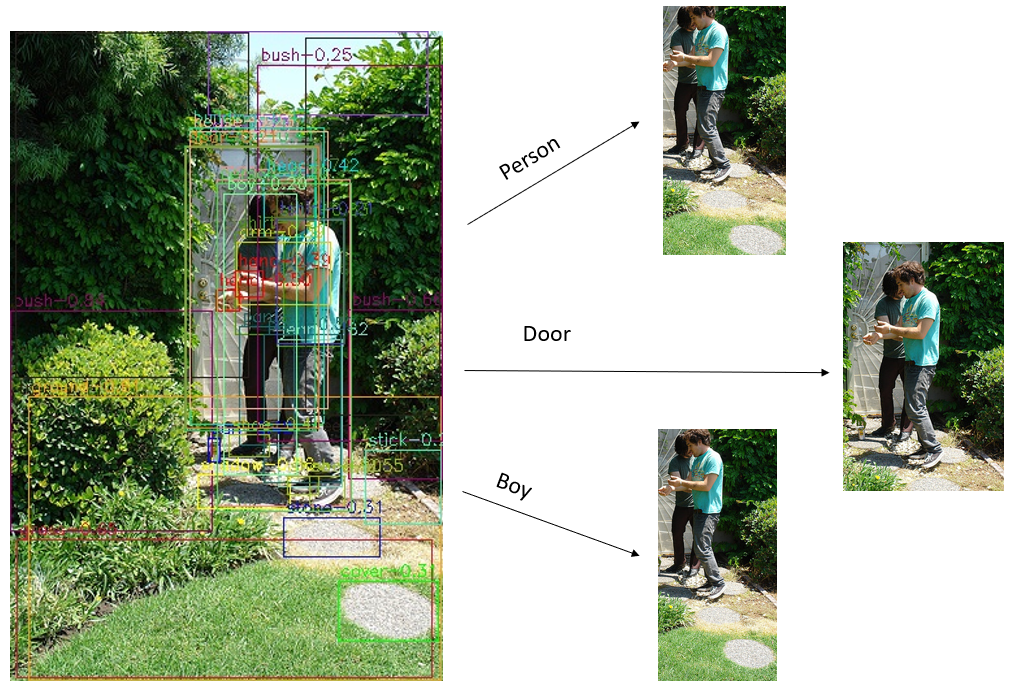
\includegraphics[width=0.8\textwidth]{risultato_detection}
\caption{Risultato del modello di Object Detection su un'immagine in cui vengono evidenziate alcune regioni sovrapposte, rumorose e ambigue che rappresentano istanze diverse (Flickr30K id 1000092795).}\label{figura:risultato_detection}
\end{figure}
Per risolvere il problema è stata utilizzata la segmentazione, la quale oltre alla classe e alla bounding box permette di determinare una maschera di segmentazione che permette di estrarre solamente l'istanza di interesse rimuovendo i pixel superflui.


In questo lavoro di tesi le risorse computazionali sono state limitate e per ottenere i risultati migliori possibili sono stati utilizzati due modelli di segmentazione già addestrati con ottime performance.
Nel dettaglio si tratta di un modello di Panoptic Segmentation allenato su \acrshort{coco} Panoptic \cite{lin2014microsoft} (composto da \acrshort{coco} instances e \acrshort{coco} stuff), il quale permette di ottenere segmentazioni delle immagini coerenti, ricche e complete.
Questo modello è in grado di predire solamente 133 classi e per aumentare il numero di oggetti riconoscibili è stato utilizzato un modello aggiuntivo di Instance Segmentation allenato su \acrshort{lvis} \cite{gupta2019lvis} (\acrlong{lvis}).
Quest'ultimo dataset è molto interessante poiché prevede 1203 categorie di oggetti ed è facilmente integrabile con \acrshort{coco}, infatti \acrshort{lvis} è un'estensione di \acrshort{coco} instances e prevede per le immagini maschere di segmentazione di qualità superiore che seguono meglio i confini degli oggetti.
Il modello di Panoptic Segmentation utilizzato è \textbf{\acrshort{detr}} \cite{carion2020end}, mentre il modello di Instance Segmentation utilizzato è una \acrshort{mask_rcnn} \cite{gupta2019lvis, he2017mask} (identificata con \textbf{Mask-\acrshort{lvis}}) allenata su \acrshort{lvis} tramite tecniche di data augmentation, poiché il dataset presenta categorie molto sbilanciate.
I due modelli insieme riescono a riconoscere 1280 classi, le quali sono state unificate gestendo eventuali sinonimi (per esempio: tv e television), le classi troppo rare e specifiche sono state raggruppate nella classe più generica (per esempio Bible è stata inserita in book),  è stata rimossa la classe più generica dai tag di classe che la contengono (per esempio dalla classe "beef (food)" è stato rimosso (food), diventando solo "beef") e le classi finali ottenute sono 1248.



Data un'immagine vengono utilizzati Mask-\acrshort{lvis} e \acrshort{detr} per estrarre le bounding box, le maschere di segmentazione e le classi degli oggetti. L'estrazione delle componenti q e v della tripla (vedere Sezione \ref{object_detection} per maggiori dettagli), per ogni istanza rilevata, è effettuata tramite le seguenti fasi:
\begin{enumerate}
\item Viene estratto l'oggetto dall'immagine di partenza utilizzando la maschera predetta e sul risultato viene utilizzata la bounding box per estrarre solo la regione di interesse. Dall'immagine originale viene rimossa l'istanza rilevata utilizzando la maschera di segmentazione affinché le prossime estrazioni non la contengano.
Inoltre, se nelle estrazioni successive la regione estratta ha più del 60\% di pixel bianchi viene presa l'immagine di partenza senza rimozioni per effettuare l'estrazione dell'oggetto segmentato, in questo modo si ottiene un buon contenuto visivo dell'oggetto riducendo le sovrapposizioni. Quindi in questa fase si ottiene una regione contenente l'oggetto segmentato con sfondo bianco;
\item La regione ottenuta precedentemente viene ridimensionata utilizzando l'interpolazione bilineare\footnote{L'interpolazione bilineare, durante il ridimensionamento e l'interpolazione di nuovi pixel, utilizza i pixel adiacenti 2x2 dell'immagine per calcolare la media ponderata utilizzata per ottenere il pixel interpolato.} \cite{jaderberg2015spatial} (questa tipologia di interpolazione è stata usata anche nel modello \acrshort{mask_rcnn} per ottenere risultati migliori, vedere sezione \ref{mask_section} per maggiori dettagli), la quale si comporta molto bene sia nei casi di riduzione (downscale) sia in quelli di aumento della dimensione (upscale) della regione. Questa fase è molto importante per la determinazione delle feature dell'oggetto;
\item Vengono estratte le feature v' della regione ridimensionata tramite il modello \acrshort{resnet} \cite{he2016deep}, quest'ultimo è stato utilizzato per unificare le rappresentazioni e perché il modello di Object Detection utilizzato usa \acrshort{resnet} come backbone. Le feature v' vengono concatenate insieme al vettore z contenente la posizione dell'oggetto. Infine, v' e z vengono concatenati per ottenere il vettore di feature della regione finale (vedere Sezione \ref{object_detection} per maggiori dettagli);
\item Viene utilizzata la label di classe predetta per ottenere il word embedding q;
\end{enumerate}
Infine, una volta che sono stati estratti tutti gli oggetti l'immagine finale pulita dalle segmentazioni viene valutata verificando se il numero di pixel non bianchi che contiene siano maggiori del 40\% rispetto ai pixel totali. Se questa condizione è rispettata allora l'immagine contenente i pixel che non sono stati segmentati viene trattata come una regione assegnandogli la classe Other e come bounding box il vettore \texttt{[0, 0, image\_width, image\_height]} (questo approccio ha preso ispirazione dal dataset \acrshort{coco} stuff, nel quale i pixel non segmentati vengono considerati nella classe Other).


La Figura \ref{figura:pipeline_segmentation} mostra l'estrazione delle feature per le istanze rilevate tramite segmentazione. Le fasi utilizzate vengono ripetute prima per tutti gli oggetti rilevati tramite il modello Mask-\acrshort{lvis} e successivamente per tutti gli oggetti rilevati tramite \acrshort{detr}, vengono effettuati in questo ordine perché la Panoptic Segmentation può rilevare classi meno specifiche e questo può portare a sovrapposizioni.
\newpage
\begin{figure}[h]
\centering
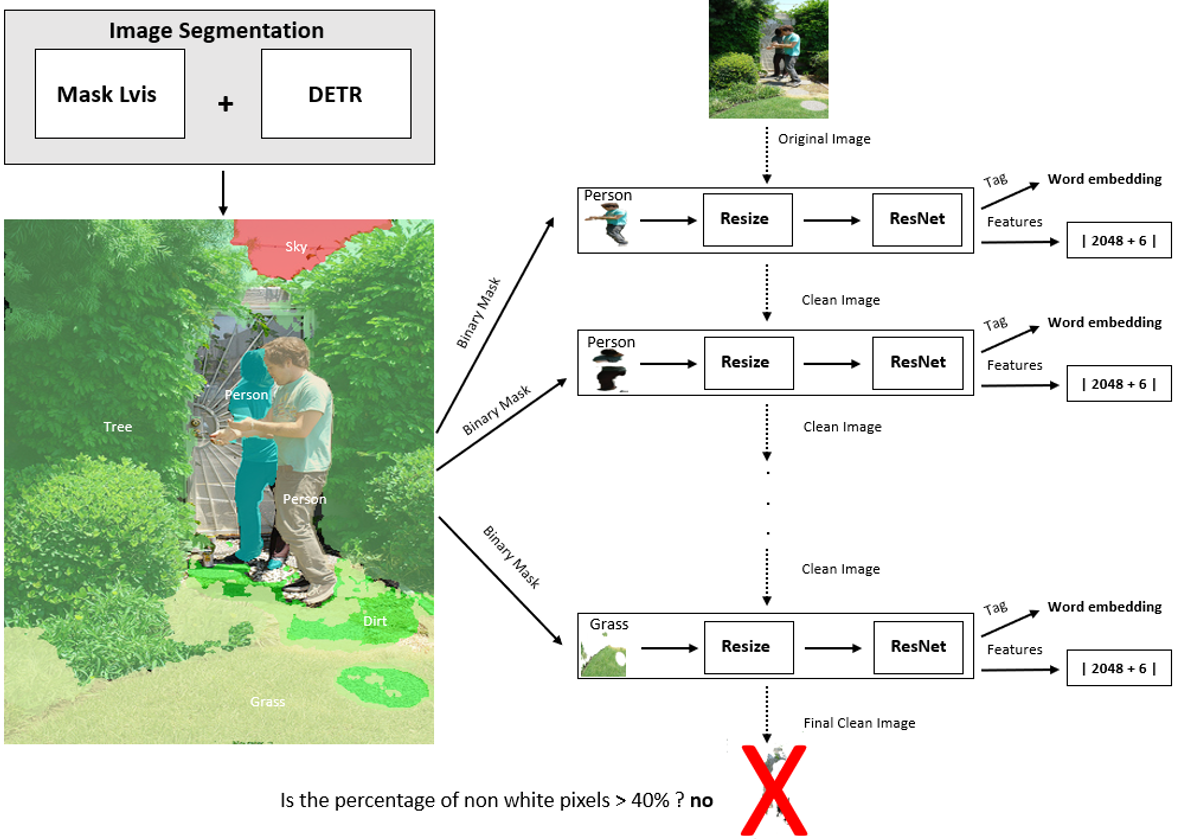
\includegraphics[width=0.95\textwidth]{pipeline_segmentation}
\caption{Illustrazione riassuntiva dell'estrazione delle feature dagli oggetti ottenuti tramite Image Segmentation.}\label{figura:pipeline_segmentation}
\end{figure}

\subsection{Combinazione tra Object Detection e Image Segmentation}\label{combinazione}
L'ensemble dei modelli di segmentazione riesce a predire meno classi rispetto al modello di Object Detection utilizzato e spesso oggetti molto importanti che sono imprescindibili per la comprensione del contenuto visivo e per la generazione della caption non vengono rilevati. La Figura \ref{figura:segmentazione_regioni_mancanti} mostra un caso in cui viene rilevata una sola regione raffigurante una persona ma all'interno dell'immagine sono presenti altri oggetti molto importanti, come la chitarra, che non vengono rilevati tramite segmentazione. 
\begin{figure}[ht!]
\centering
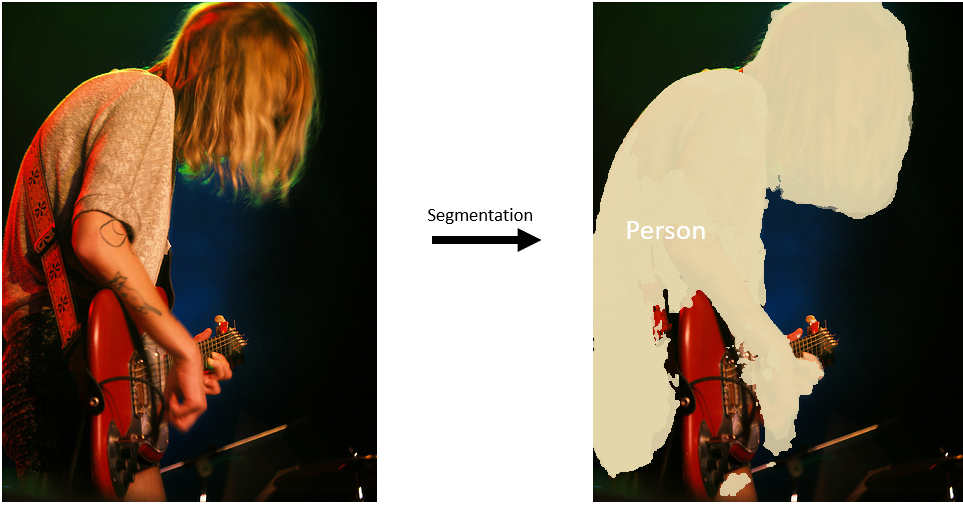
\includegraphics[width=0.9\textwidth]{segmentazione_regioni_mancanti.png}
\caption{Illustrazione in cui si può notare la mancanza della rilevazione di oggetti importanti per comprendere il contenuto visivo dell'immagine e per generare una caption di buona qualità. Id immagine Flickr30K: 6184270681}\label{figura:segmentazione_regioni_mancanti}
\end{figure}
La segmentazione in media riesce a estrarre 14 oggetti con un numero massimo di istanze rilevate in una singola immagine pari a 71 e con un minimo di 1. Mentre, il modello di Object Detection rileva in media 44 oggetti con un numero massimo di istanze rilevate in una singola immagine pari a 100 e con un minimo di 10.
Inoltre, l'ensemble dei modelli di segmentazione a volte ha difficoltà nella predizione delle classi corrette.



Il primo problema precedentemente individuato è stato risolto includendo le regioni predette tramite Object Detection non rilevate tramite segmentazione. Una regione estratta dal modello di Object Detection risulta non rilevata se il suo vettore rappresentante la bounding box non ha cosine similarity maggiore di 0.98 con il vettore della bounding box di nessun oggetto estratto tramite l'ensemble di Image Segmentation.


Mentre, il secondo problema è stato risolto tramite una pipeline di correzione delle classi estratte tramite segmentazione, dove vengono recuperate le regioni simili estratte tramite Object Detection.
La \textit{pipeline di correzione delle classi} prevede le seguenti fasi:
\begin{enumerate}
    \item Per ogni oggetto rilevato tramite Image Segmentation viene creato un insieme di regioni simili rilevate tramite Object Detection utilizzando la cosine similarity applicata sui vettori rappresentanti la bounding box e un valore di similitudine minimo utilizzato per filtrare. Dall'insieme creato vengono estratti i tre oggetti più simili basandosi sulle tre modalità seguenti:
    \begin{enumerate}[leftmargin=2.5cm,label=Metodo \arabic*:]
        \item recupera l'oggetto considerando l'etichetta di classe più frequente e tra questi prende quello con la confidenza di predizione più elevata;
        \item prende l'oggetto con la bounding box che ottiene il punteggio di cosine similarity maggiore;
        \item prende l'oggetto il cui vettore delle feature ottiene il valore di cosine similarity più alto considerando il vettore delle feature dell'oggetto segmentato che si sta valutando;
    \end{enumerate}
    In tutti i metodi se ci sono più oggetti candidati che sopravvivono, tra questi viene preso quello con la confidenza di predizione maggiore.
    Quindi questa fase termina restituendo un insieme composto da tre oggetti (uno per ogni metodo);
    \item Su ogni oggetto rilevato come candidato viene calcolato uno score pesato che considera la similarità tra le feature, la similarità tra i word embedding e la confidenza di predizione della classe rilevata tramite Object Detection. La formula \ref{score} viene utilizzata per calcolare il punteggio che viene assegnato a ogni oggetto.
\end{enumerate}
\begin{equation}\label{score}
        score = features\_similarity  \cdot  0.6 + words\_similarity  \cdot  0.3 + conf  \cdot  0.1
\end{equation}
Infine, viene presa la classe dell'oggetto che ottiene lo score più alto, la quale andrà a sostituire la classe dell'oggetto estratto tramite segmentazione che si sta valutando.
Nello score è stata privilegiata la similarità tra i vettori delle feature.


\section{Language Model}
Il modello linguistico utilizzato si basa su \acrshort{bert} \cite{devlin2018bert} e si chiama \textbf{\acrshort{oscar}$_+$} \footnote{\url{https://github.com/microsoft/Oscar}}, questo modello è stato pre-addestrato su un grande dataset D composto dai dataset vision-language esistenti, tra cui quelli di Image Captioning: \acrshort{coco} \cite{lin2014microsoft}, Conceptual Captions (CC) \cite{sharma2018conceptual}, SBU captions \cite{ordonez2011im2text}, Flickr30k \cite{young2014image}; i dataset di Visual Question Answering: GQA \cite{hudson2019gqa}, VQA \cite{goyal2017making}, VG-QA; infine, viene utilizzata una porzione del dataset OpenImages di Image Tagging. In totale, il dataset finale è composto da 5.65 milioni di immagini uniche e da 8.85 milioni di triple testo-tag-immagine, le quali sono state estratte tramite il modello di Object Detection.
Il pre-training di \acrshort{oscar}$_+$ è stato effettuato utilizzando la funzione obiettivo riportata nell'equazione \ref{funzione_obiettivo} composta dalla combinazione di due loss function diverse.

\begin{equation}\label{funzione_obiettivo}
L_{Pre-training} = L_{MTL} + L_{CL3}
\end{equation}

La funzione obiettivo definita precedentemente è calcolata considerando l'input del modello come una composizione di due prospettive diverse:
\begin{equation*}
x \stackrel{\Delta}{=} [\textcolor{red}{w}, \textcolor{green}{q}, \textcolor{green}{v}] = [\textcolor{red}{w}, \textcolor{red}{q} , \textcolor{green}{v}] \stackrel{\Delta}{=} x'
\end{equation*}
dove il rosso indica la rappresentazione del linguaggio e il verde la rappresentazione dell'immagine.
Inoltre, x indica la \textit{modality view} usata per distinguere le rappresentazioni tra un testo e un'immagine; mentre $x'$ è la \textit{dictionary view} usata per distinguere i due diversi spazi semantici in cui l'input è rappresentato.


La dictionary view usa la \textbf{\acrfull{mtl}}, in questa modalità i token dei tag degli oggetti (o answer per i dati di visual question answering) e i token delle parole delle caption (o question per i dati di visual question answering) condividono lo stesso spazio semantico linguistico, mentre le feature delle regioni dell'immagine si trovano nello spazio semantico visivo. La \acrlong{mtl} per il pre-training è applicata sulla sequenza discreta di token, la quale è definita come $h \stackrel{\Delta}{=} [w, q]$. A ogni iterazione, viene mascherato casualmente ogni token di input in h con una probabilità del 15\% e il token $h_i$ viene sostituito con un token speciale \texttt {[MASK]}. L'obiettivo dell'addestramento è prevedere questi token mascherati basandosi sui token circostanti $h_{\setminus i}$ e su tutte le feature dell'immagine v, minimizzando la log-likelihood negativa:
\begin{equation*}
L_{MTL} = -E_{(v, h) \sim D} \hspace{0.1cm} log \hspace{0.1cm} p(h_i|h_{\setminus i},v)
\end{equation*}
Questa funzione di perdita è simile a quella usata da \acrshort{bert}, in questa variante la parola o l'etichetta mascherata deve essere recuperata da ciò che la circonda, con la partecipazione delle informazioni aggiuntive dell'immagine che aiutano a definire i word embedding appresi nel contesto della visione.


La modality view usa la \textbf{\acrfull{lcl3}}, nella quale vengono definite due tipologie di triple inquinate (non abbinate) per i due tipi di campioni di allenamento. Le triple inquinate sono composte da ($w'$, q, v) = \{caption, image-tags, image-features\} per i dati di image captioning e image tagging, e (w, $q'$, v) = \{question, answer, image-features\} per i dati di visual question answering (il carattere con $'$ indica la componente inquinata). Successivamente viene usato un fully-connected (FC) layer f($\cdot$) in cima a esso come un classificatore con 3 possibili valori, il quale prevede: se la tripla è abbinata (c = 0), contiene una w inquinata (c = 1) o contiene una q inquinata (c = 2).
Quindi, il modello è addestrato a distinguere triple vere o false e questa funzione di perdita è definita come:
\begin{equation*}
L_{CL3} = -E_{(w, q, v; c) \sim \widetilde{D}} \hspace{0.1cm} log \hspace{0.1cm} p(c|f(w, q, v))
\end{equation*}
dove il dataset (w, q, v; c) $\in \widetilde{D}$ contiene il 50\% di triple corrette, il 25\% di triple con w inquinata e il 25\% di triple con q inquinata. 
Le triple inquinate prevedono la sostituzione di q con una probabilità del 50\% con una sequenza di tag o answer diversa campionata casualmente dal dataset; mentre, per w inquinata la sostituzione avviene sulle caption e question.


La funzione di perdita definita consente di ottenere delle performance superiori quando viene effettuato il fine-tuning sul task specifico.

\begin{figure}[ht]
\centering
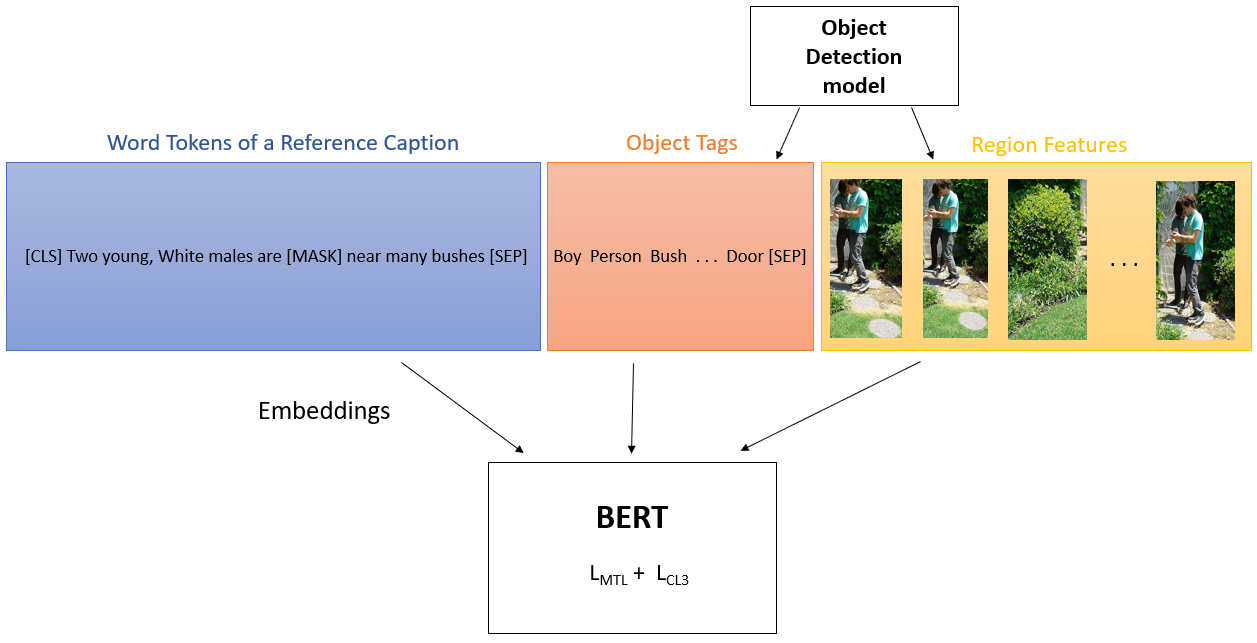
\includegraphics[width=0.99\textwidth]{architettura}
\caption{Illustrazione riassuntiva del pre-training del modello \acrshort{oscar}$_+$, il fine-tuning sul task di Image Captioning prevede come loss solo la \acrshort{mtl} e le componenti q e v della tripla possono essere estratte utilizzando il modello di Object Detection, l'ensemble dei modelli di segmentazione o la combinazione tra detection e segmentation.}
\end{figure}

\subsection{Fine-Tuning}

Il modello \acrshort{oscar}$_+$ pre-addestrato viene utilizzato per l'Image Captioning effettuando fine-tuning mantenendo lo stesso input composto da triple, ma la funzione di perdita è composta solamente dalla \acrlong{mtl}. Le componenti q e v della tripla possono essere estratte tramite il modello di Object Detection, tramite l'ensemble dei modelli di segmentazione o tramite la combinazione tra Object Detection e Image Segmentation. La self-attention mask di \acrshort{bert} viene vincolata affinché un token della didascalia possa partecipare solo ai token prima della sua posizione per simulare un processo di generazione unidirezionale.

 
%Recentemente è stato dimostrato \cite{rennie2017self} che il training basato su metriche non differenziabili genera bias durante l'inferenza e non consente di ottimizzare il modello direttamente sulle metriche per il compito da svolgere. Quindi sono state sviluppate tecniche che risolvono questi problemi e le metodologie in questione si basano su approcci di reinforcement learning.
Oltre al fine-tuning precedente per migliorare l'apprendimento a livello di sequenza viene effettuato un ulteriore fine-tuning del modello ottenuto applicando un approccio di ottimizzazione basato sul \acrlong{rl} chiamato \acrfull{scst} \cite{rennie2017self}, vedere Sezione \ref{scst} per maggiori dettagli. Esistono diversi modelli \cite{anderson2018bottom, zhou2020unified, li2020oscar, zhang2021vinvl} che hanno utilizzato questo approccio ottenendo miglioramenti significativi in fase di test. In questo approccio il modello di Image Captioning è considerato come un agente i cui parametri determinano una politica.
A ogni passo temporale, l'agente esegue la politica per scegliere un'azione, cioè la previsione della prossima parola nella frase generata. Una volta raggiunta la fine della sequenza l'agente riceve una ricompensa e lo scopo dell'addestramento è di ottimizzare i parametri dell'agente per massimizzare la ricompensa prevista.
La ricompensa viene determinata utilizzando la metrica \acrshort{cider} (vedere Sezione \ref{cider} per maggiori dettagli), la quale si correla bene con il giudizio umano ed è stata pensata appositamente per il task di Image Captioning.
% Tramite questa tecnica la ricompensa è normalizzata rispetto a un valore di base per ridurre la varianza.  ??????
L'approccio di \acrlong{rl} non viene applicato fin da subito perché risulta difficile per questa procedura ottenere miglioramenti significativi in un tempo accettabile (per esempio con le risorse a nostra disposizione una singola epoca con \acrshort{scst} richiede circa undici ore), quindi viene effettuato prima un altro fine-tuning usando tecniche standard e poi viene utilizzato \acrshort{scst}.
\subsection{Inferenza}
Durante l'inferenza, prima vengono rilevate e codificate le regioni dell'immagine e i tag degli oggetti rilevati tramite una delle modalità specificate nella Sezione \ref{visual_encoder}. Successivamente il modello \acrshort{oscar}$_+$ utilizza le feature estratte per effettuare la generazione della caption, la quale inizia inserendo un token \texttt{[MASK]} e campionando un token dal vocabolario basato sull'output di verosimiglianza condizionato dalle codifiche delle regioni, dei tag e dalle parole precedenti della sequenza (se è la prima parola la sequenza è composta solo dal token di inizio frase). Successivamente, il token \texttt{[MASK]} viene sostituito con il token campionato e un nuovo token \texttt{[MASK]} viene aggiunto per la previsione della parola successiva. Il processo di generazione termina quando il modello linguistico produce il token \texttt{[STOP]}. La decodifica della sequenza di output viene effettuata tramite uno degli algoritmi indicati nella Sezione \ref{algoritmi_decodifica}.